\documentclass{standalone}

\RequirePackage{times}
\RequirePackage{amsmath}
\RequirePackage{amssymb}
\RequirePackage[T1]{fontenc}

\usepackage{tikz}
\usepackage{xcolor}
\usepackage{pgfplots}
\pgfplotsset{compat=1.16}
\usetikzlibrary{arrows}
\usetikzlibrary{backgrounds,scopes}

\definecolor{background}{RGB}{79, 192, 202}

\begin{document}
	\begin{tikzpicture}[line cap=round,line join=round,x=1.0cm,y=1.0cm]
		%clip area
		\clip(-0.5,0) rectangle (11,6.4);
		
		%coordinate system etc.
		\begin{axis}[
			x=1.0cm,y=1.0cm,
			axis lines=middle,
			ymajorgrids=true,
			xmajorgrids=true,
			xmin=-0.5,
			xmax=10.5,
			ymin=-2.7,
			ymax=3.7,
			xtick={0.0,1.0,...,10.0},
			ytick={-2.0,-1.0,...,5.0},
			xlabel={$x$},
			ylabel={$y$},
			ticklabel style={fill=white,text opacity=1,fill opacity=0.66,inner sep=3pt,rounded corners=5pt},
			label style={fill=white,text opacity=1,fill opacity=0.66,inner sep=3pt,rounded corners=5pt},]
			\begin{scope}[on background layer]
				\node[inner sep=0pt,outer sep=0pt,anchor=north west] at (-2.0,3.7) {
					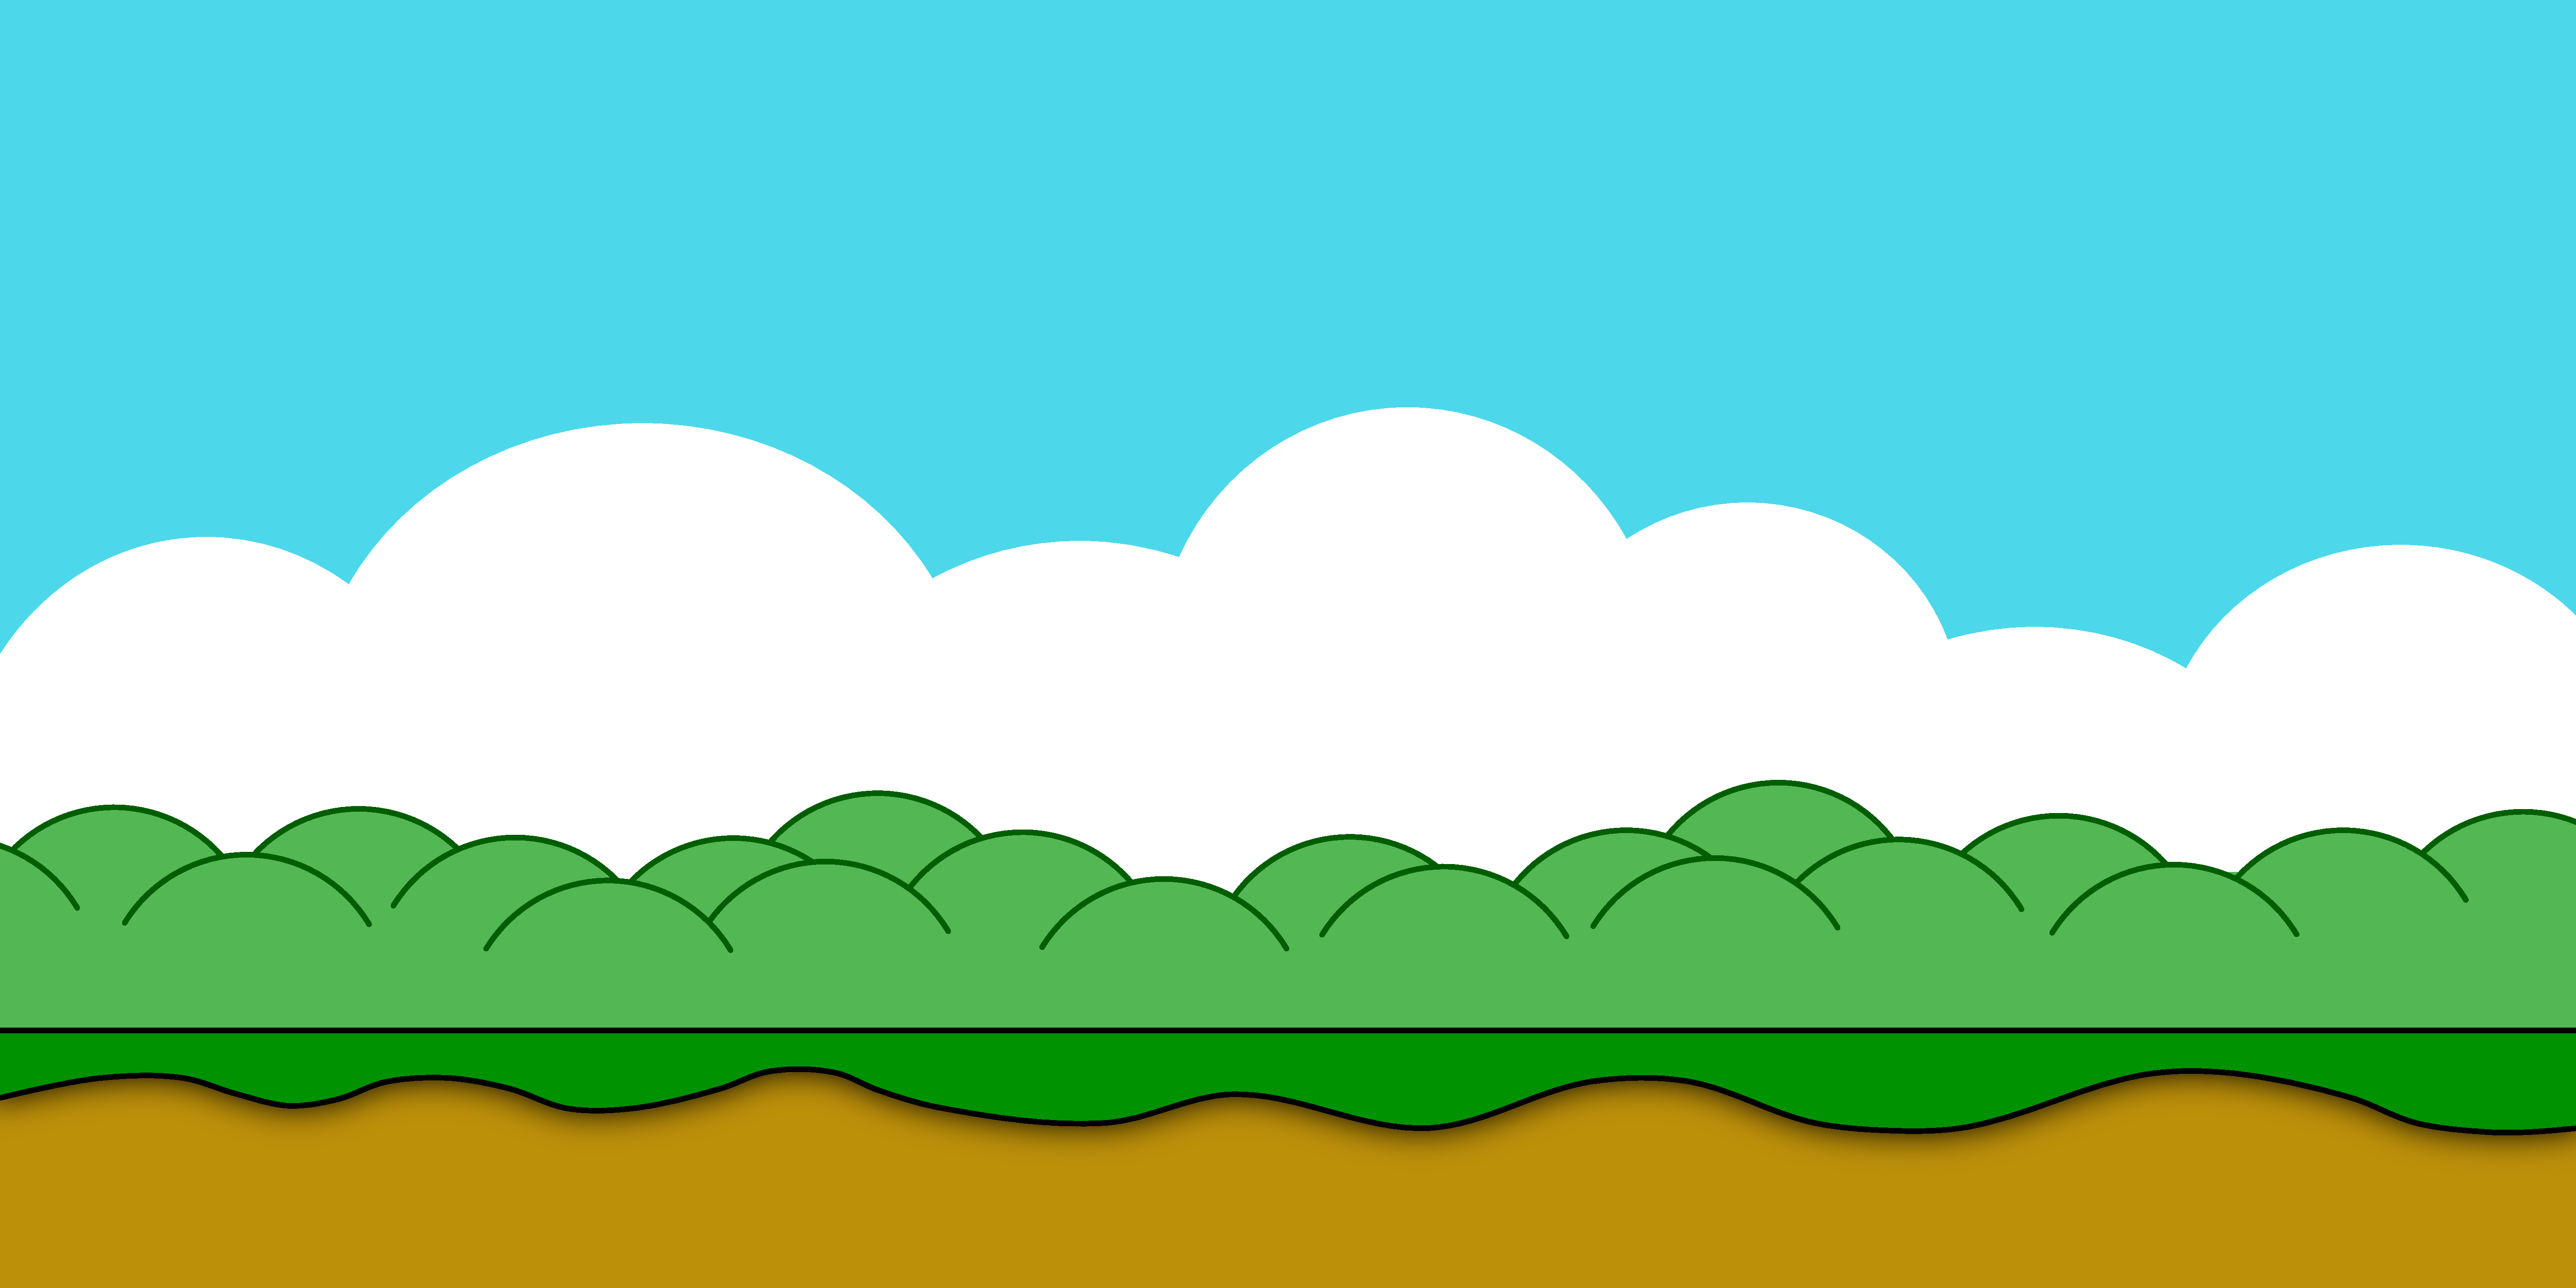
\includegraphics[width=14cm]{bg}
				};
			\end{scope}
			%commands
			\newcommand{\interval}[3]{
				\begin{scope}[on background layer]
					\node[inner sep=0pt,outer sep=0pt,anchor=north west]
					at (#1-0.5,#2) {
						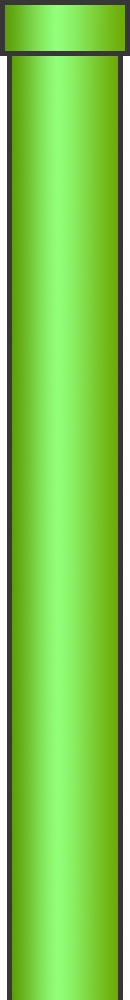
\includegraphics[interpolate=false,width=1cm]{pipe}
					};
					\node[inner sep=0pt,outer sep=0pt,anchor=south west]
					at (#1-0.5,#3) {
						\scalebox{1}[-1]{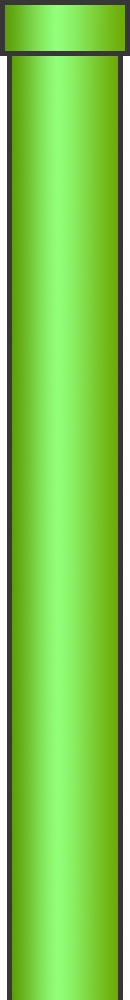
\includegraphics[interpolate=false,width=1cm]{pipe}}
					};
				\end{scope}
				\draw[{|-|},color=red,ultra thick] (#1,#2)--(#1,#3);
			};
			\newcommand{\solution}[1]{
				\draw[ultra thick] plot[mark=*,mark size=2] coordinates {#1}; 
			};
		
			%test data
			\interval{2}{1}{3};
			\interval{4}{2}{3};
			\interval{7}{0}{2};
			\interval{9}{-2}{-1};
			\solution{(0,0)(4,2)(9,-1)(10,0)}
			
			%bird
			\node[inner sep=0pt,outer sep=0pt]
			at (0,0) {
				\rotatebox{0}{
\includegraphics[interpolate=false,width=0.5cm]{bird}}
			};
		\end{axis}
	\end{tikzpicture}
\end{document}